\pagebreak
\subsection{Electrical Design}

\subsubsection{Block Diagram}
\label{sec:4.5.1}
The architecture of the electrical design is shown in figure \ref{fig:electronic-architecture}.

\begin{figure}[H]
	\centering
	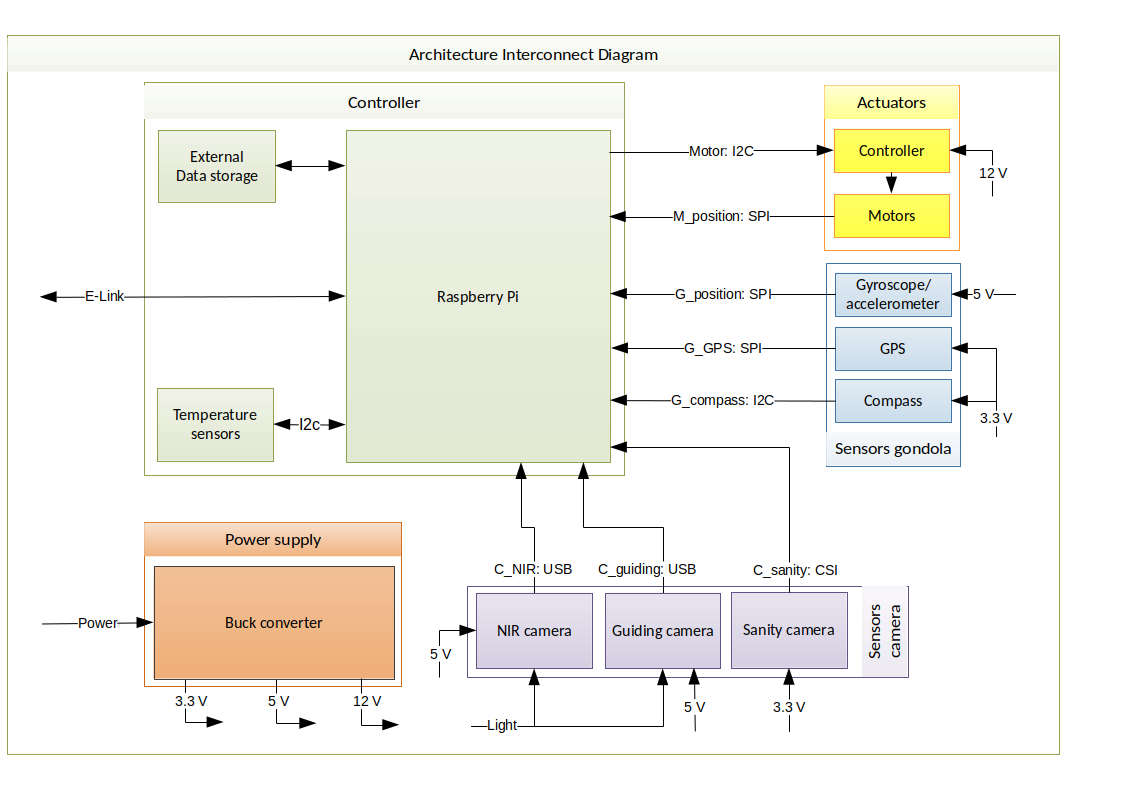
\includegraphics[width=\textwidth]{4-experiment-design/img/electrical/ArchitectureInterconnect.png}
	\caption{An architecture diagram of the electronics.}
	\label{fig:electronic-architecture}
\end{figure}

%\subsubsection{Critical Component/Part A}

%\subsubsection{Critical Component/Part B}

%\subsubsection{Critical Component/Part C}

\subsubsection{Schematic}
See Appendix c.

\subsubsection{PCB Layout}
There will be three PCB:s, which are listed below:

\begin{itemize}
	\item 	Power system \& Motor control
	\item	Gyroscopes
	\item 	Sensors
\end{itemize}

The two PCB:s, Power system \& Motor control  and Gyroscopes, will be located in the electronics box. They will be placed on top of each other. %, see figure \ref{fig:electronic-box}

%\begin{figure}[H]
%	\centering
%	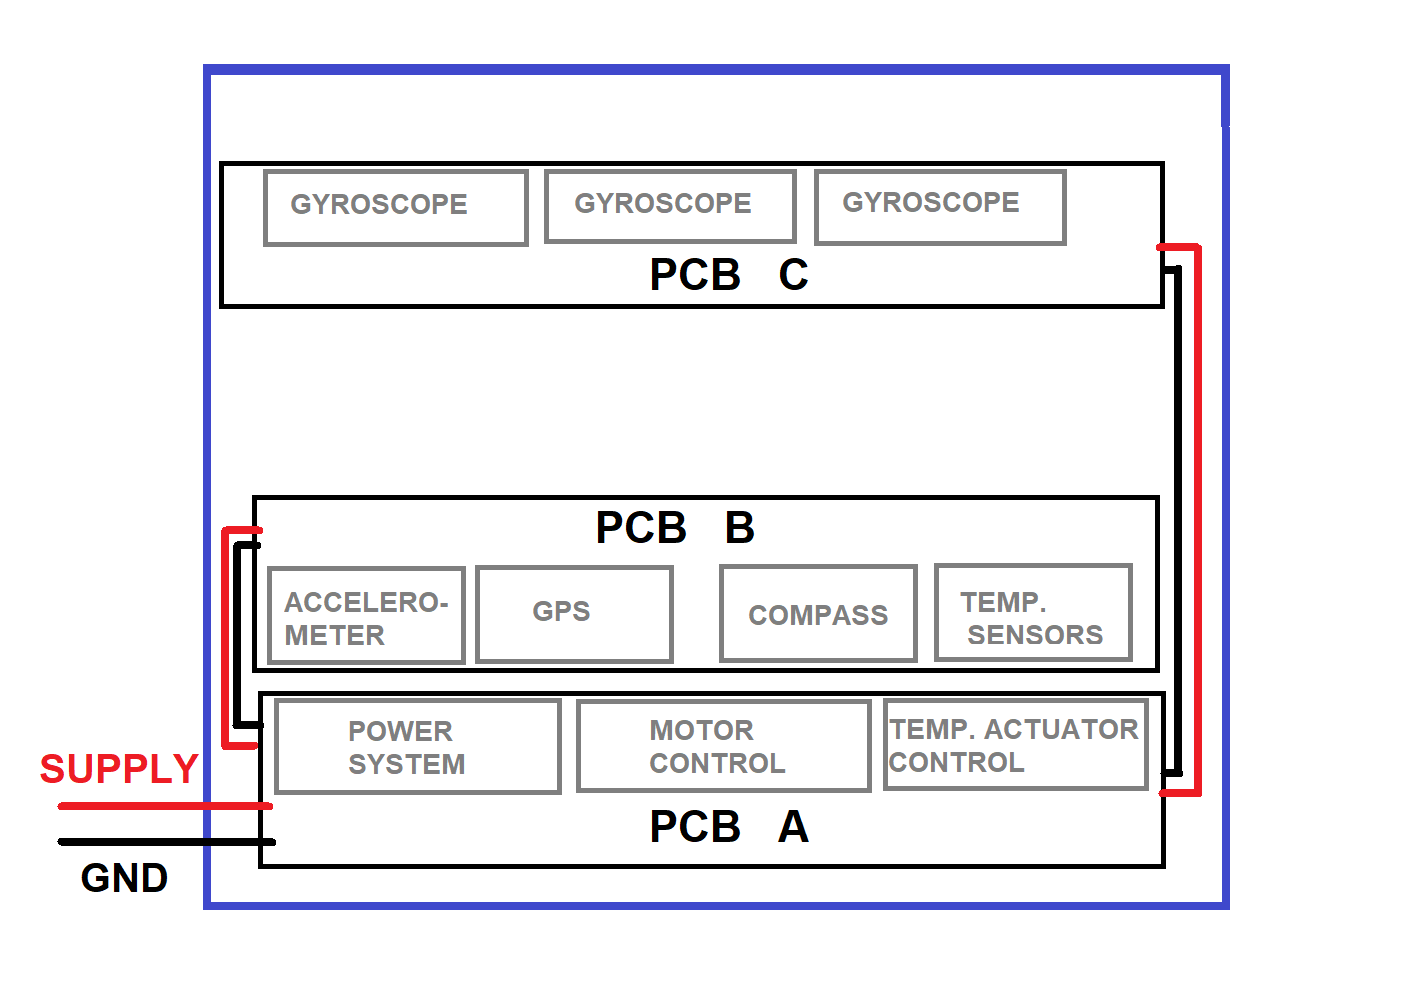
\includegraphics[width=\textwidth]{4-experiment-design/img/electrical/ElectricalBox.png}
%	\caption{An architecture diagram of the electronics.}
%	\label{fig:electronic-box}
%\end{figure}


The third PCB will be placed in its own second electronics box. Because this PCB includes the sensors as GPS, accelerometers and magnetometer. Thus the PCB should not be too close to the other PCBs or the DC motors due to disturbances, such as for example magnetic field changes. The schematics of all the PCBs can be found in appendix C.
\raggedbottom
